\documentclass[10pt,a4paper]{article}
\usepackage[margin=1.6cm,top=1.2cm,bottom=1.3cm]{geometry}
\usepackage{graphicx,booktabs,amsmath,microtype,xcolor,enumitem,caption}
\usepackage[hidelinks]{hyperref}
\usepackage{mathptmx}
\captionsetup{font=small,labelfont=bf,skip=3pt}
\setlist{nosep,leftmargin=1.2em}
\setlength{\parskip}{2pt}\setlength{\parindent}{0pt}
\makeatletter
\renewcommand\section{\@startsection{section}{1}{\z@}{6pt plus 2pt}{2pt}{\normalfont\large\bfseries}}
\makeatother
\pagestyle{plain}

\begin{document}
\begin{center}
{\Large\bfseries A Compact NAFNet U-Net for Blind, General-Purpose Image Restoration}\\[3pt]
{\normalsize Mini Competition: A Small Generative Model for Image Denoising --- Technical Report}\\[2pt]
{\small Sachin (P26CS0010) \quad$\cdot$\quad Code: \url{https://github.com/ritchi-e/GenAI_mini}}
\end{center}

\vspace{-4pt}
\section{Summary}
We submit a 6.5\,M-parameter, \textbf{4.45\,GFLOPs} (fvcore, input $1{\times}3{\times}256{\times}256$) convolutional restoration network that maps one corrupted $256{\times}256{\times}3$ image to a restored $256{\times}256{\times}3$ \texttt{uint8} image. The model is \emph{blind}: it receives no information about the type or strength of the corruption. Generalisation comes from training on an effectively infinite stream of randomly composed degradation chains (13 noise/blur/compression families with random order, severity and mixing) over natural, medical and low-light images. On our held-out validation set of 119 images, it raises PSNR from 21.5 to \textbf{30.6\,dB}, SSIM to \textbf{0.830} and lowers DISTS to \textbf{0.179}.

\textbf{Generative formulation.} The network is a conditional generative model of the clean image given the corrupted one, $\hat{x} = G_\theta(y) \approx \mathbb{E}[x \mid y]$, trained on synthetic pairs drawn from a hand-designed, randomised forward corruption process $y \sim q(y\mid x)$. We chose this single-step conditional generator over iterative diffusion sampling deliberately: FLOPs are ranked equally with quality, and one forward pass of our network costs roughly what a single denoising step of a diffusion U-Net costs. The perceptual (DISTS) fine-tuning stage moves the output away from the pure posterior mean towards sharper, more realistic texture.

\section{Architecture}
A 4-level U-Net built from \textbf{NAFBlocks} (Chen et al., \emph{Simple Baselines for Image Restoration}, ECCV 2022). Each block: LayerNorm $\rightarrow$ 1$\times$1 conv $\rightarrow$ 3$\times$3 depth-wise conv $\rightarrow$ SimpleGate ($x_1 \odot x_2$) $\rightarrow$ simplified channel attention $\rightarrow$ 1$\times$1 conv, then a gated FFN; both branches use learned residual scales initialised to zero. NAFBlocks contain no nonlinear activation functions and give state-of-the-art quality per FLOP on denoising and deblurring. Down-sampling uses stride-2 2$\times$2 convs, up-sampling uses 1$\times$1 conv + PixelShuffle, and encoder features are added (not concatenated) to the decoder. A \textbf{global residual} makes the network predict a correction to the input, so clean regions are preserved. Most compute sits at $1/8$ and $1/16$ resolution, which keeps FLOPs low while giving the large receptive field that motion and defocus blur require. Only conv, element-wise and mean ops are used, so fvcore and ptflops count the model completely.

\begin{table}[h]\centering\small
\caption{Submitted configuration (\texttt{configs/small.yaml}).}
\begin{tabular}{lllll}\toprule
Width & Encoder blocks (levels 1--4) & Middle & Decoder blocks & Params / FLOPs @256$^2$\\\midrule
24 (24$\to$384 ch.) & 1, 1, 2, 4 & 4 & 1, 1, 1, 1 & 6.53\,M / 4.45\,GFLOPs (fvcore), 4.52\,GMACs (ptflops)\\\bottomrule
\end{tabular}\end{table}
\vspace{-6pt}

\section{Training data}
All sources are public research or Creative Commons datasets. Large images are cut into 384\,px tiles at scales 1, $\tfrac12$ and $\tfrac14$ (the down-scaled tiles imitate whole scenes resized to 256$^2$); medical images are resized to 256\,px. Training samples domains with weights natural 0.6 / medical 0.3 / low-light 0.1 (45{,}340 source tiles in total).
\begin{itemize}
\item \textbf{Natural}: DIV2K train HR (800 photos, images 0001--0740 used for training).
\item \textbf{Medical}: MedMNIST+ 224\,px (PneumoniaMNIST chest X-ray, OrganCMNIST CT, BreastMNIST ultrasound, RetinaMNIST fundus; CC BY 4.0) and Brain-Tumor-MRI T1/T2 slices (MIT).
\item \textbf{Low-light}: LOL dataset normal-light images, plus on-the-fly darkening of any image (below).
\end{itemize}

\section{Degradations used during training}
Corruptions are synthesised \emph{on the fly}, so no corrupted image is ever seen twice. For each patch a random chain is applied in physical image-formation order:
\begin{enumerate}
\item \textbf{Blur} ($p{=}0.45$): anisotropic \textbf{Gaussian} ($\sigma$ 0.3--3.5), linear or curved \textbf{motion} blur (3--25\,px), \textbf{defocus} disk (radius 1--6).
\item \textbf{Chromatic aberration} ($p{=}0.2$): lateral R/B scaling and shift, optional single-channel blur.
\item \textbf{Resolution loss} ($p{=}0.12$): down/up-resizing by $\times$1.3--4 with random interpolation.
\item \textbf{Noise} ($p{=}0.8$; a second noise is mixed in with $p{=}0.2$): \textbf{Gaussian} ($\sigma$ 1--55, colour or luminance), \textbf{Poisson} (peak 5--500), \textbf{speckle}, \textbf{salt-and-pepper} (0.2--10\%), Rician (MRI), uniform, spatially correlated (film grain / demosaicing), row/column banding.
\item \textbf{JPEG} quality 5--95 ($p{=}0.35$), bit-depth quantisation ($p{=}0.05$), late impulse noise ($p{=}0.06$).
\item Rounding to the \texttt{uint8} grid, matching the competition inputs.
\end{enumerate}
About 3\% of samples are left clean so the model learns not to over-smooth clean inputs. Content augmentation: flips/90$^\circ$ rotations, grayscale conversion ($p{=}0.08$) and \textbf{low-light simulation} ($p{=}0.15$: the clean target is darkened with gamma 1--2.2 and gain 0.08--0.6 before corruption). The families beyond the brief's list (Rician, banding, correlated noise, resizing) and the random combinations are intended to cover the undisclosed held-out corruptions.

\section{Training objective and schedule}
\vspace{-8pt}
\[
\mathcal{L} = \underbrace{\mathcal{L}_\text{Charbonnier}}_{\text{PSNR}} + 0.2\,\underbrace{(1-\text{SSIM})}_{\text{SSIM}} + 0.05\,\underbrace{\|\mathcal{F}(\hat x)-\mathcal{F}(x)\|_1}_{\text{sharpness after blur}} + \lambda_\text{D}\,\underbrace{\text{DISTS}(\hat x, x)}_{\text{perceptual}},\qquad \lambda_\text{D}\in\{0,\,0.05\}
\]
Each term targets one evaluation axis. AdamW ($\beta{=}(0.9,0.9)$), learning rate $10^{-3}$ with 2k-iteration warm-up and cosine decay to $10^{-6}$, gradient clipping 0.5, bf16 autocast, and an \textbf{EMA} of the weights (decay 0.999); the EMA weights are submitted. Progressive training for 200k iterations on one NVIDIA A30: iterations 0--150k with 128\,px patches, batch 32; 150k--185k with 256\,px patches (the true test size), batch 16; 185k--200k at 256\,px with the DISTS term switched on ($\lambda_\text{D}{=}0.05$). The checkpoint with the best balanced validation score $\text{PSNR}/40 + \text{SSIM} - \text{DISTS}$ is kept (here the final one).

\section{Results}
\textbf{Validation set.} 119 image pairs never used in training: 60 DIV2K photos (0741--0800), 32 MedMNIST \emph{test} images, 12 Brain-MRI \emph{test} images and 15 darkened LOL-eval images, each with its own random degradation chain (fixed seed). Metrics follow the competition protocol (\texttt{skimage} PSNR/SSIM and official DISTS on \texttt{uint8} 256$^2$ images).

\begin{table}[h]\centering\small
\begin{minipage}[t]{0.46\linewidth}\centering
\caption{Held-out validation set (final EMA weights).}
\begin{tabular}{lrrrrr}\toprule
Domain & $n$ & PSNR$_\text{in}$ & PSNR$\uparrow$ & SSIM$\uparrow$ & DISTS$\downarrow$\\\midrule
Natural & 60 & 19.69 & 25.96 & 0.764 & 0.205\\
Medical & 44 & 22.10 & 34.08 & 0.891 & 0.136\\
Low-light & 15 & 27.26 & 38.86 & 0.915 & 0.203\\\midrule
\textbf{All} & 119 & 21.53 & \textbf{30.59} & \textbf{0.830} & \textbf{0.179}\\\bottomrule
\end{tabular}

\end{minipage}\hfill
\begin{minipage}[t]{0.51\linewidth}\centering
\caption{Single corruptions written independently of the training pipeline (mean of 4 validation images; PSNR dB / SSIM, input $\rightarrow$ output).}
\begin{tabular}{lcc}\toprule
Corruption & PSNR & SSIM\\\midrule
Gaussian $\sigma{=}25$ & 21.0 $\rightarrow$ 31.7 & 0.42 $\rightarrow$ 0.91\\
Gaussian $\sigma{=}50$ & 15.5 $\rightarrow$ 28.6 & 0.23 $\rightarrow$ 0.83\\
Poisson (peak 20) & 19.8 $\rightarrow$ 31.3 & 0.46 $\rightarrow$ 0.90\\
Salt \& pepper 5\% & 17.6 $\rightarrow$ 40.7 & 0.46 $\rightarrow$ 0.99\\
Speckle $\sigma{=}0.2$ & 25.3 $\rightarrow$ 34.3 & 0.74 $\rightarrow$ 0.95\\
Gaussian blur $\sigma{=}2$ & 26.7 $\rightarrow$ 30.9 & 0.74 $\rightarrow$ 0.90\\
Motion blur 15\,px & 25.2 $\rightarrow$ 27.7 & 0.68 $\rightarrow$ 0.80\\
JPEG $q{=}10$ & 26.9 $\rightarrow$ 27.9 & 0.78 $\rightarrow$ 0.83\\
Chromatic aberration & 22.8 $\rightarrow$ 35.3 & 0.70 $\rightarrow$ 0.95\\
Blur + noise + JPEG & 25.0 $\rightarrow$ 27.5 & 0.61 $\rightarrow$ 0.80\\
Clean input (identity) & --- $\rightarrow$ 53.5 & 1.00 $\rightarrow$ 1.00\\\bottomrule
\end{tabular}
\end{minipage}
\end{table}

The DISTS fine-tune (185k$\to$200k) cut validation DISTS from 0.198 to 0.179 ($-$10\%) for a 0.04\,dB PSNR and 0.001 SSIM cost, the best trade under per-axis ranking. Clean inputs pass through almost unchanged (53.5\,dB), so the model does not hallucinate or over-smooth.

\begin{figure}[h]\vspace{-4pt}\centering
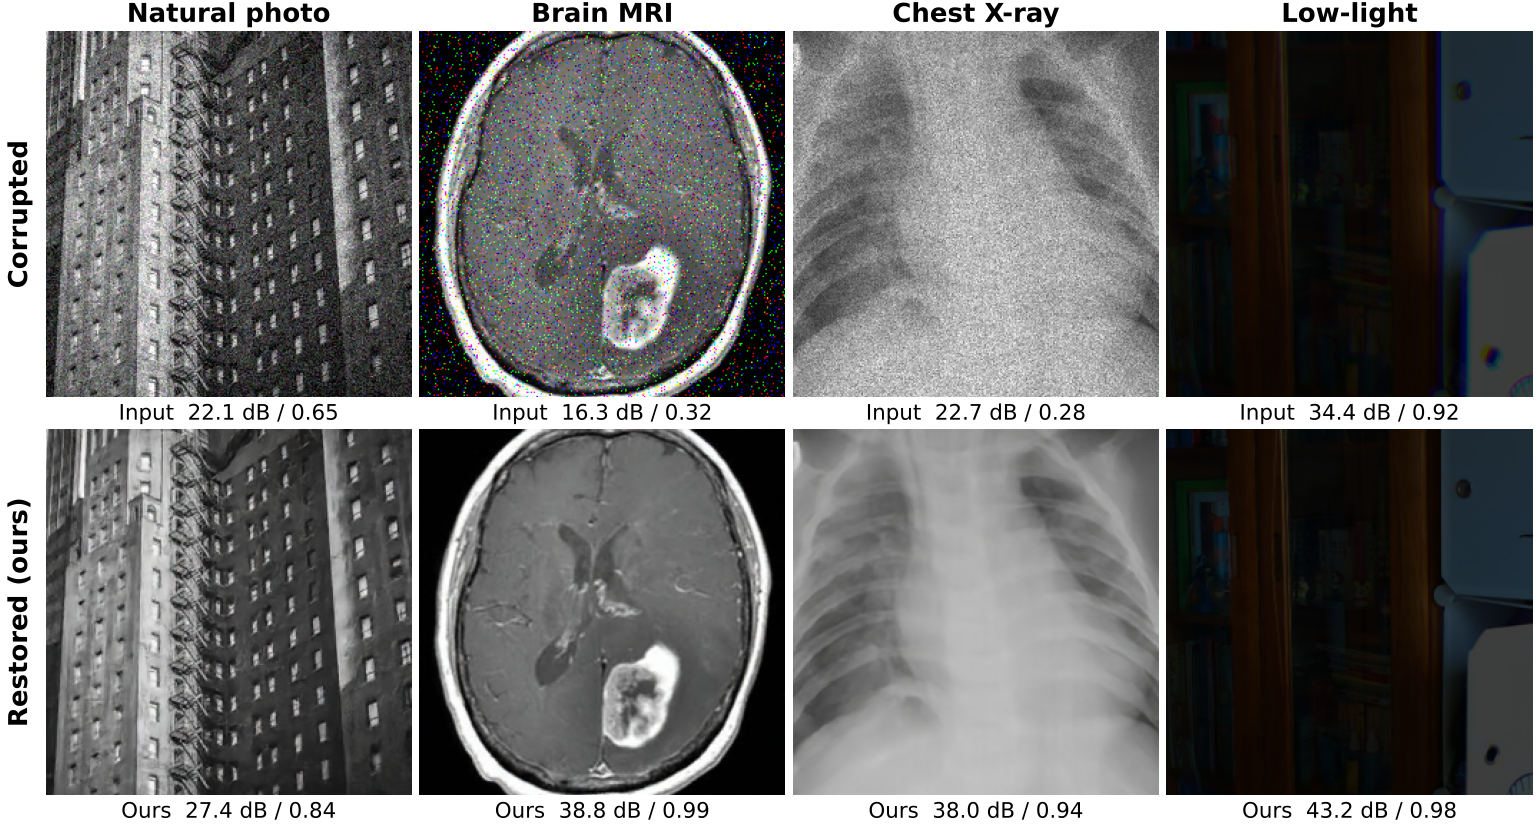
\includegraphics[width=0.83\linewidth]{fig_examples.png}
\caption{Validation examples across the three content domains (labels: PSNR / SSIM against the clean ground truth).}
\end{figure}

\section{Limitations}
\begin{itemize}
\item The validation corruptions come from the same family of generators as training, so the held-out score will likely be lower than 30.6\,dB; Table~3 (independent corruptions) is the more honest estimate.
\item Strong motion blur and very low-quality JPEG are the hardest cases (+2.5 and +1.0\,dB). At high noise, fine natural texture is smoothed (e.g.\ animal fur).
\item Global photometric changes outside the training families (haze, contrast loss) are not corrected.
\end{itemize}

\section{Submission contents}
\texttt{weights/model.pth} (PyTorch \texttt{\{"state\_dict","arch"\}}, fp32) and \texttt{weights/model.onnx} (opset 17, verified against PyTorch, max.\ abs.\ diff.\ $4{\times}10^{-7}$). Inference: \texttt{python inference.py --input <img|dir> --output <dir>}; output is always \texttt{uint8} in $[0,255]$. FLOPs: \texttt{python count\_flops.py --weights weights/model.pth}. Training, data and Slurm scripts are included.

\end{document}
